\chapter{Arkitektur}

I dette afsnit beskrives systemets arkitektur for hardware og software. Arkitekturens formål er at tildele roller til de enkelte hardware og software komponenter. Når denne arkitektur er fast sat er det muligt at designe systemet i detaljer. Arkitekturen illustreres i hardware-delen i Blok definition diagram (BDD), Internal blok diagram (IBD) og en blokbeskrivelse, der indeholder uddybende beskrivelse af blokkene i BDD'et. For Software-delen anvendes også et BDD, som bruges til at illustrere hovedblokkene.

\section{Hardware}
\subsection{Blok definition diagram}

Blok definition diagrammet



\begin{figure}[H] 
\centering
{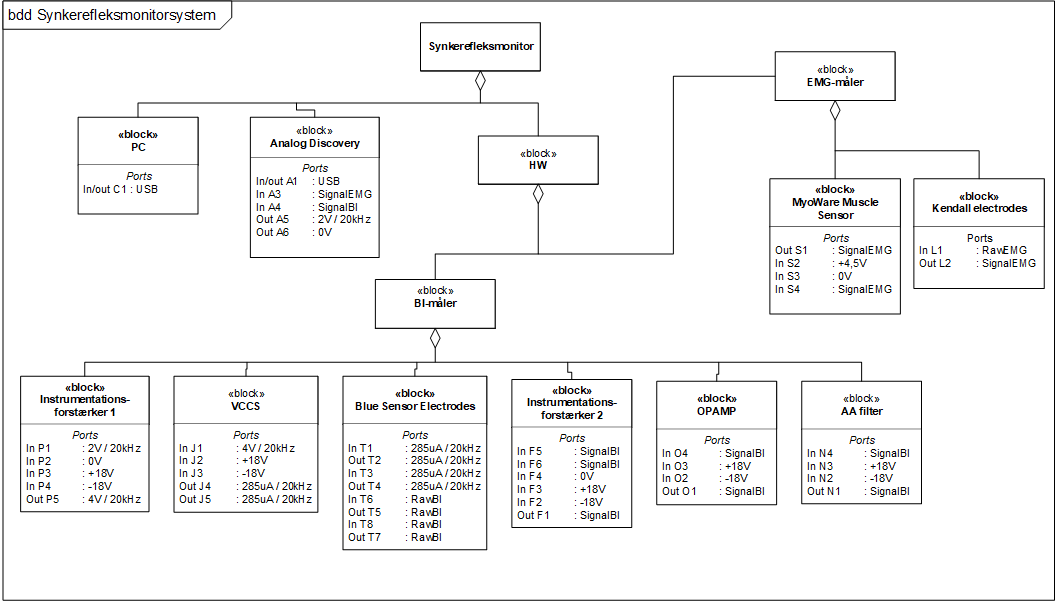
\includegraphics[width=\linewidth]
{Figure/BDD}}
\caption{Figuren viser de enkelte komponenter, som hardware-delen består af. Overordnet består
systemet af en Bioimpedansmåler, en EMG-måler og enhed som både bruges til som
dataopsamlingsenhed og funktionsgenerator. Udover det er der en PC blok.}
\label{procesVoresASE}
\end{figure}